\documentclass[12pt]{beamer}
\usetheme{default} 

\setbeamertemplate{navigation symbols}{} %gets rid of navigation symbols
\setbeamertemplate{footline}{} %gets rid of bottom navigation bars
\setbeamertemplate{footline}[page number]{} %use this for page numbers

\setbeamertemplate{footline}{%
  \raisebox{5pt}{\makebox[\paperwidth]{\hfill\makebox[10pt]{\scriptsize\insertframenumber~~}}}}

\setbeamertemplate{itemize items}[circle] %round bullet points
\setlength\parskip{10pt} % white space between paragraphs

\usepackage{wrapfig}
\usepackage{subfig}
\usepackage{setspace}
\usepackage{enumerate}
\usepackage{graphicx}
\usepackage{amsmath}
\usepackage{amsfonts}
\usepackage{amssymb}
\usepackage{amsthm}
\usepackage[UKenglish]{isodate}
\usepackage{tikz}
\usepackage{pgfplots}
\usepackage{natbib}
\usepackage{hyperref}
\hypersetup{
    colorlinks=true, 
    urlcolor=blue
}
\def\checkmark{\tikz\fill[scale=0.4](0,.35) -- (.25,0) -- (1,.7) -- (.25,.15) -- cycle;} 

% allow drawing arrows
\usetikzlibrary{arrows}
\tikzstyle{arrow}=[draw, -latex] 

% bracketing shortcuts
\newcommand{\paren}[1]{\left(#1\right)}
\newcommand{\sqbracket}[1]{\left[#1\right]}
\newcommand{\cbracket}[1]{\left\{#1\right\}}
\newcommand{\abs}[1]{\left\lvert#1\right\rvert}
\newcommand{\norm}[1]{\left\lVert#1\right\rVert}
% set up the argmin operator, argmax
\DeclareMathOperator*{\argmin}{arg\,min}
\DeclareMathOperator*{\argmax}{arg\,max}

\newcommand{\myframe}[1]{\begin{frame} \frametitle{#1}}

% New itemize environment, with spaces
\newenvironment{spaceitemize}
{ \begin{itemize}
    \setlength{\itemsep}{10pt}
    \setlength{\parskip}{0pt}
    \setlength{\parsep}{0pt}     }
{ \end{itemize}                  } 


% the preamble
\title{Day 1, Session 1: Overview}
\author{Jessica Williams-Nguyen and Brian D. Williamson}
\institute{EPI/BIOST Bootcamp 2017}
\date{22 September 2017}

% Start the document
\begin{document}
% The title page
\begin{frame}
\titlepage
\end{frame}

\myframe{Welcome!}
\begin{spaceitemize}
\item Welcome to the EPI/BIOST Bootcamp!
\item For today:
\begin{spaceitemize}
\item Our backgrounds
\item Introduction to course content for EPI 511 and BIOST 508, 511
\item Overview of this course
\item Some skills and resources for success in graduate school
\item Math Skills I
\end{spaceitemize}
\end{spaceitemize}
\end{frame}

\myframe{Our backgrounds: Jessica}
\begin{spaceitemize}
\item Fifth year PhD student, Epidemiology
\item Research interests: Infectious diseases and zoonoses, Genetic epidemiology and advanced methods
\item Dissertation cohort: CFAR Network of Integrated Clinical Sites (CNICS)
\end{spaceitemize}
\end{frame}

\myframe{Our backgrounds: Brian}
\centering
%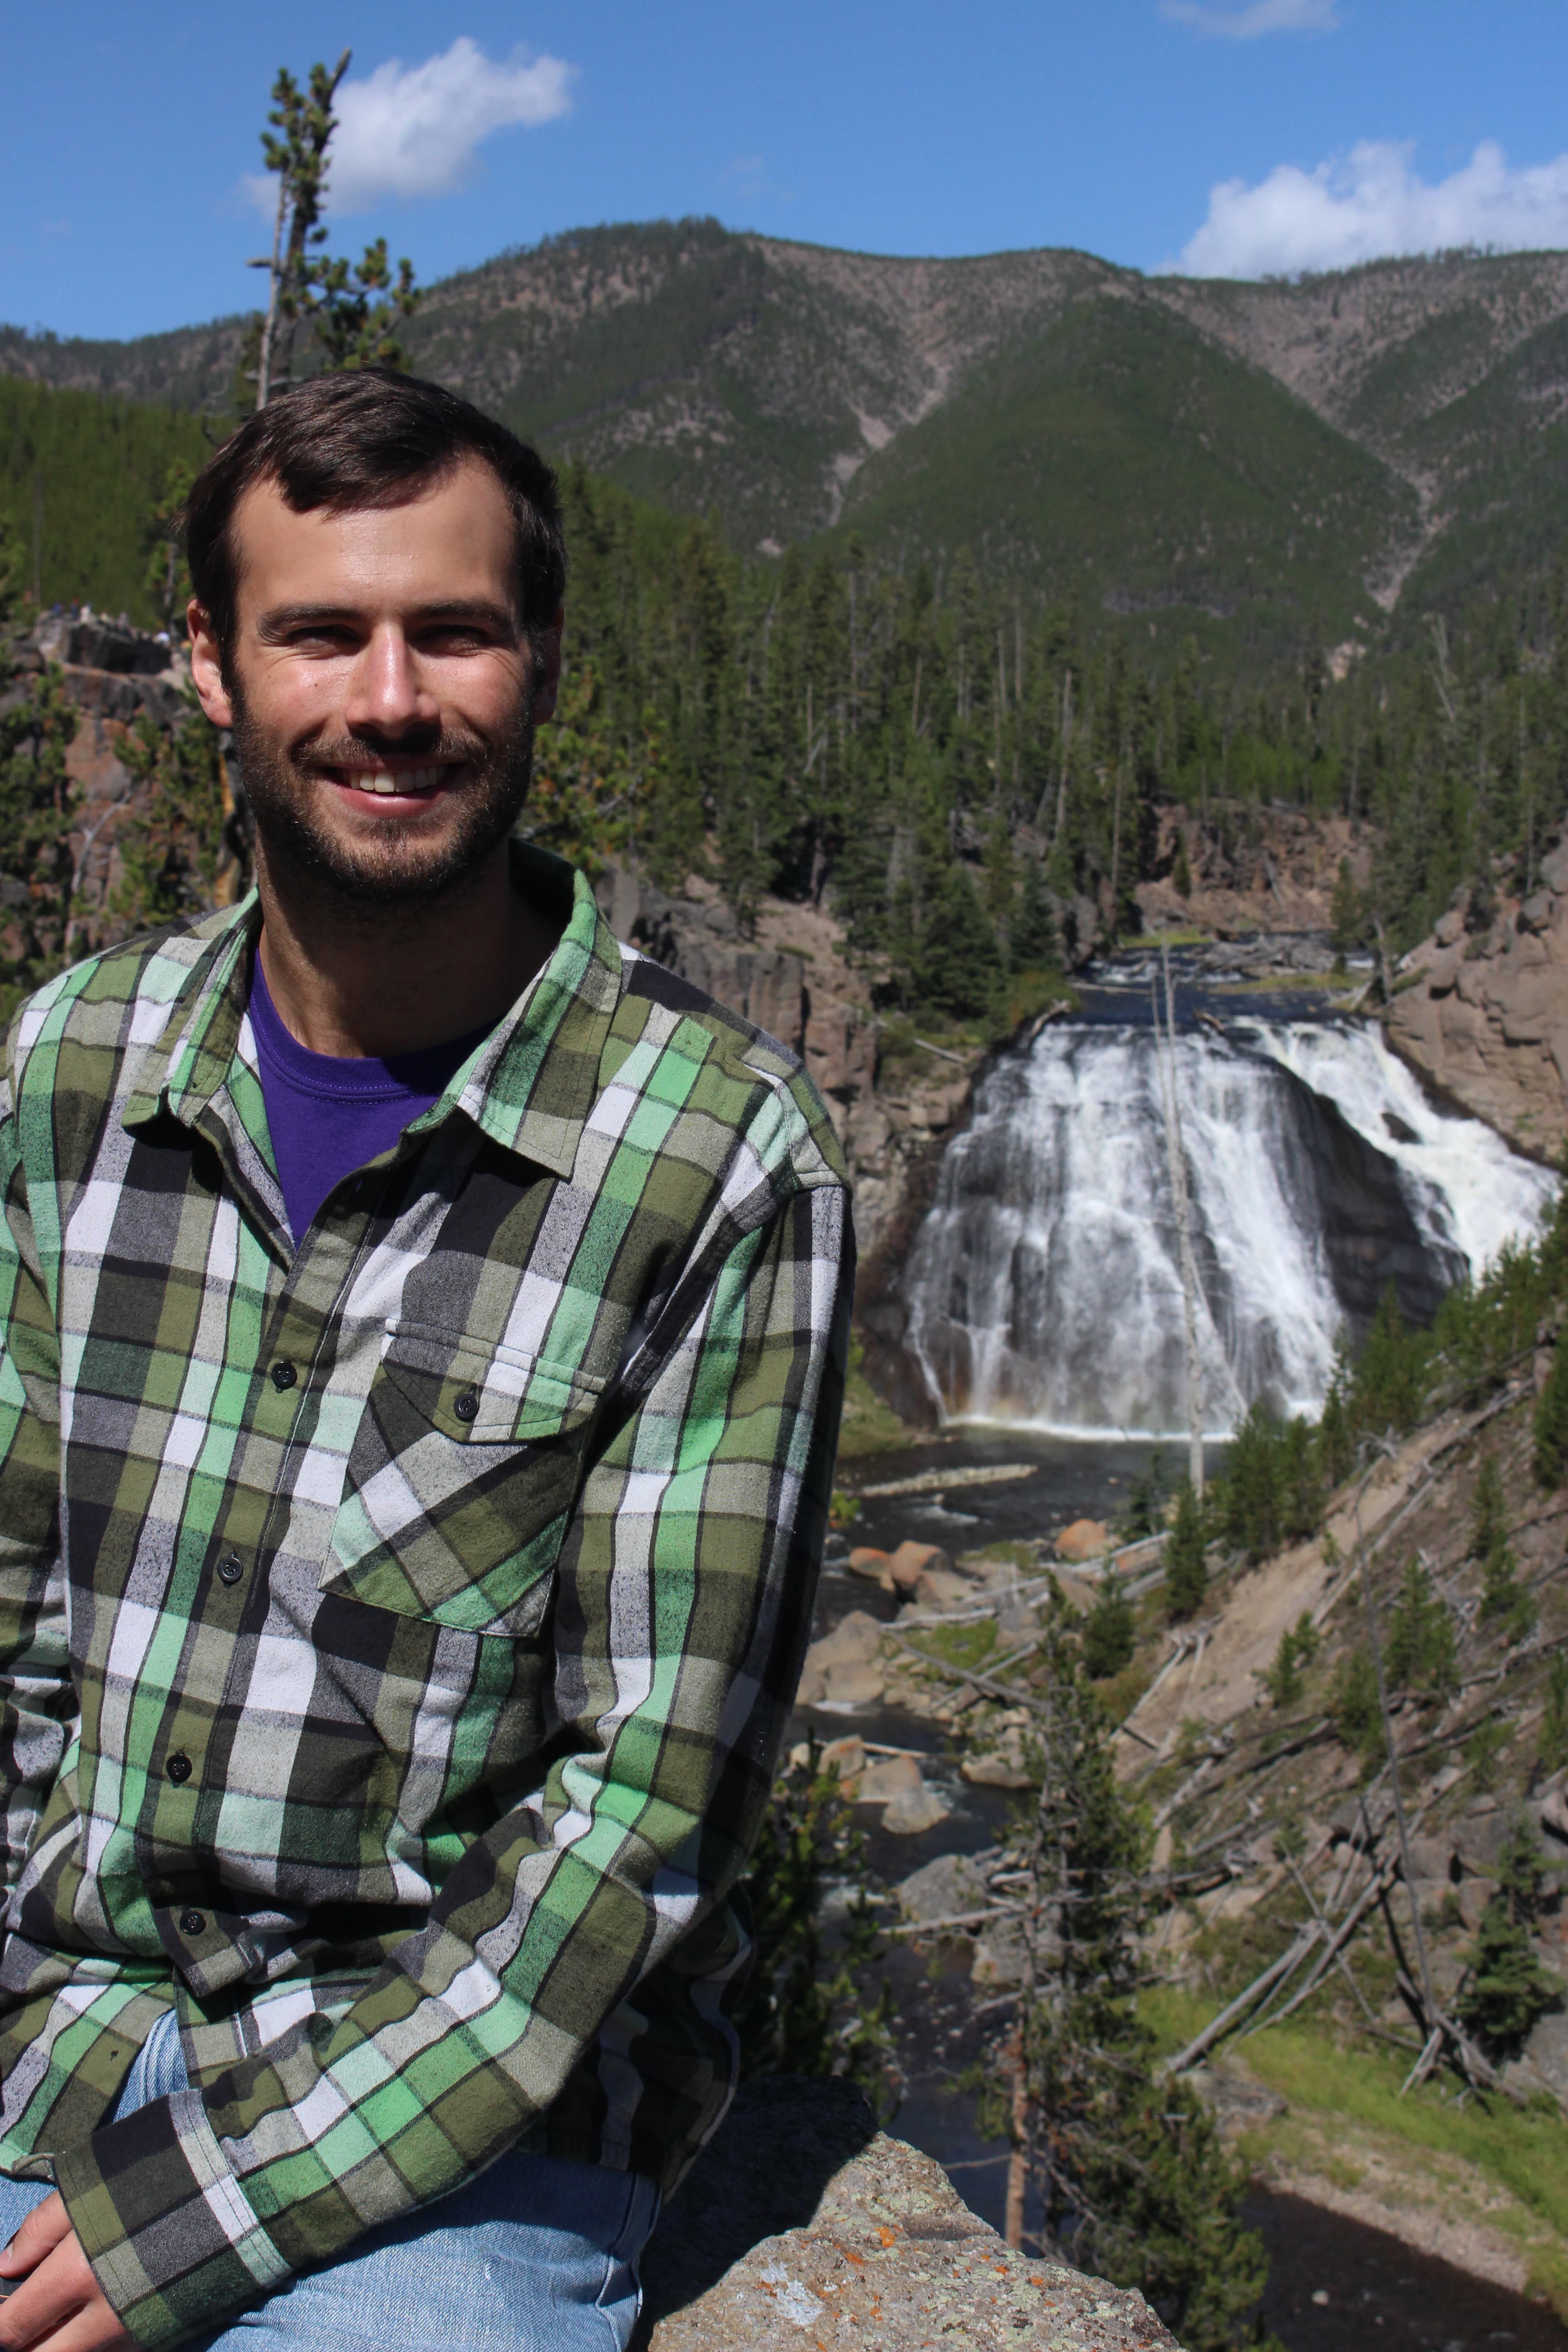
\includegraphics[width = .25\textwidth]{yellowstone-min.jpg}
\begin{spaceitemize}
\item Fourth year PhD student, Biostatistics
\item TA for BIOST 511 (Fall 2017)
\item Research interests: High-dimensional statistics and inference, HIV/AIDS
\item RA: HIV prevention clinical trials
\end{spaceitemize}
\end{frame}

\myframe{Intro to course content: BIOST 511 \small (from Jim Hughes, PhD)}
\begin{spaceitemize}
\item Objective: provide students with an understanding of basic concepts and methods of statistical inference in the health sciences
\item Some major topics:
\begin{spaceitemize}
\item Data description, exploratory data analysis
\item Basic issues in study design
\item Probability concepts and models
\item Statistical inference - estimation and hypothesis testing
\item Categorical data analysis
\item Introduction to regression analysis
\end{spaceitemize}
\end{spaceitemize}
\end{frame}

\myframe{Intro to course content: BIOST 511}
\begin{spaceitemize}
\item Only pre-requisite is basic algebra
\item However, R will be used to teach some of the concepts and analyze data
\item Depending on the instructor, will cover logs/exponents in data analysis
\end{spaceitemize}
\end{frame}

\myframe{Intro to course content: BIOST 508 \small (from Jim Hughes, PhD)}
\begin{spaceitemize}
\item Pre-requisites: basic algebra, EPI 511 or 512
\item Similar to BIOST 511 in spirit, but 
\begin{spaceitemize}
\item assumes you will not go on to BIOST 512 (includes multiple regression, ANOVA) or BIOST 513 (includes logistic regression, classification)
\item slightly less in-depth treatment than 508, but covers a few more topics (e.g., sample size calculation)
\item assumes EPI 511 or 512 content (e.g., skips some study design issues)
\end{spaceitemize}
\end{spaceitemize}
\end{frame}
\myframe{Intro to course content: EPI 511/512}
\begin{spaceitemize}
\item Objective: provide students with an understanding of basic epidemiologic concepts and methods in the health sciences 
\item Some major topics:
\begin{spaceitemize}
\item Defining and calculating major measures of disease frequency
\item Describe major sources of bias in epidemiologic research (e.g., confounding or selection bias), and ways to evaluate and reduce bias
\item Interpret results of an epidemiologic study
\item Evaluate integrity and comparability of data
\end{spaceitemize}
\end{spaceitemize}
\end{frame}

\myframe{Intro to course content: EPI 511/512}
\begin{spaceitemize}
\item Describe major epidemiologic research study designs
\item Define and calculate measures of association, and modifications of association
\end{spaceitemize}
\end{frame}

\myframe{Overview of the bootcamp}
All sessions are in this room, \textcolor{blue}{T--747}
\begin{spaceitemize}
\item Today: overview, Math Skills I
\begin{spaceitemize}
\item Order of Operations
\item Fractions, Percentages, and Decimals
\item Algebra and cross-tabulation
\end{spaceitemize}
\item Monday, 25 September (2--5:30pm): Math Skills II
\begin{spaceitemize}
\item Graphs
\item Logarithms and exponents
\item Word problems
\end{spaceitemize}
\end{spaceitemize}
\end{frame}

\myframe{Overview of the bootcamp}
\begin{spaceitemize}
\item Tuesday, 26 September (8--10:30am): R! 
\begin{spaceitemize}
\item Live demo: installing R and RStudio
\item R basics
\item Live demo: the RStudio environment
\item Accessing help files
\end{spaceitemize}
\end{spaceitemize}
\end{frame}

\myframe{Skills for success: class preparation}
\begin{spaceitemize}
\item Do readings (lecture notes, textbook) before coming to class
\item Start homework early
\item Go to class, and participate if possible!
\end{spaceitemize}
\end{frame}

\myframe{Skills for success: study groups}
\begin{spaceitemize}
\item Start early
\item Try to form study groups with people of mixed backgrounds and programs
\item Keep tabs on how members of the group are performing
\item Be careful not to plagiarize
\end{spaceitemize}
\end{frame}

\myframe{Skills for success: office hours}
\begin{spaceitemize}
\item Not just for homework help!
\item Bring corrected tests and homework to review
\item Go over concepts in the reading
\end{spaceitemize}
\end{frame}

\myframe{Skills for success: bolstering basic skills}
\begin{spaceitemize}
\item We're providing a refresher, but you may need outside help
\item Seek tutoring (early!)
\item Use online resources (e.g., Khan Academy)
\end{spaceitemize}
\end{frame}

\myframe{Skills for success: quarters move fast!}
\begin{spaceitemize}
\item Don't put off homework/reading/studying
\item The first midterm tends to be a wake-up call, but the pace picks up after it --- no time to catch up
\item Second quarter assumes mastery of the first quarter's material
\item Seek out disability accommodation early (\url{http://depts.washington.edu/uwdrs/})
\end{spaceitemize}
\end{frame}

\myframe{Skills for success: language and wording}
\begin{spaceitemize}
\item Epi, particularly, is very language-heavy
\item Pay attention to how specific words are used
\item If you are not fluent in English, consider setting up additional help early
\end{spaceitemize}
\end{frame}

\myframe{Skills for success: tips on coming recently from undergrad}
\begin{spaceitemize}
\item If coming from semester school: quarters are much faster!
\item Imposter syndrome --- remember that the UW chose you!
\item Balancing an RA/TA with coursework will likely be an adjustment
\item UW's approach may be different from that of your undergrad
\end{spaceitemize}
\end{frame}

\myframe{Skills for success: tips if you've been out of school for a while}
\begin{spaceitemize}
\item Schedule yourself more time at first than you might expect you need to complete work
\item The field may have advanced since you were in school
\item UW's approach may be different than where you worked or earned your Master's/undergraduate degree
\end{spaceitemize}
\end{frame}

\myframe{Homework for the weekend}
\begin{spaceitemize}
\item Visit the GitHub page for this bootcamp (\url{http://bit.ly/SPHbootcamp})
\begin{spaceitemize}
\item Download the slides and other materials using the green ``Clone or Download'' button (choose download)
\item Updated material may be posted to the site; re-download if necessary
\end{spaceitemize}
\item Try to bring a laptop for Tuesday's R session
\end{spaceitemize}
\end{frame}


\end{document}
